\documentclass[12pt]{Qual}
\usepackage{preamble}

\name{Kayla Orlinsky}
\course{Complex Analysis Exam}
\term{Fall 2013}
\hwnum{Fall 2013}

\begin{document}

\begin{problem} $\,$
Compute $$\int_0^\infty\frac{\log^2x}{1+x^2}dx$$
\end{problem}


\begin{solution}$\,$
We will use ``Ol' Faithful'' the contour around the upper half plane avoiding the origin since every branch cut of $\log x$ intersects $0$.

Then we take any branch which does not intersect the upper half plane (including the real line).
\begin{center}
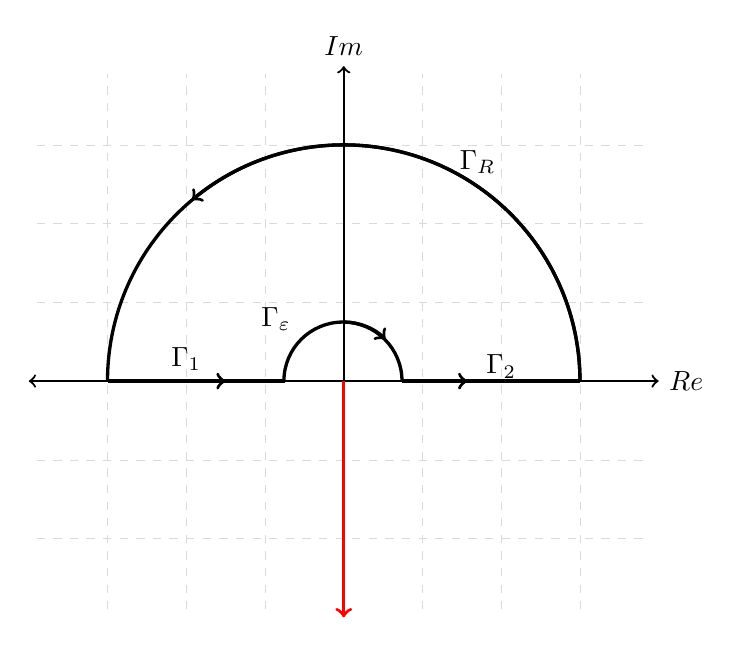
\begin{tikzpicture}
\draw[help lines, color=gray!30, dashed] (-3.9,-2.9) grid (3.9,3.9);
\draw[->,very thick] (3,0) arc (0:130:3cm);
\draw[very thick] (3,0) arc (0:180:3cm) node[above,yshift=2.5cm,xshift=4.7cm]{$\Gamma_R$};
\draw[->,very thick] (0,0.75) arc (90:45:0.75cm);
\draw[very thick] (0.74,0) arc (0:180:0.75cm) node[above,yshift=0.5cm,xshift=-0.1cm]{$\Gamma_\varepsilon$};
\draw[->,very thick] (0.74,0) -- (1.57,0);
\draw[very thick] (0.75,0) -- (3,0) node[above,yshift=-0.1cm,xshift=-1cm]{$\Gamma_2$};
\draw[->,very thick] (-3,0) -- (-1.5,0);
\draw[very thick] (-0.74,0) -- (-3,0) node[above,yshift=0cm,xshift=1cm]{$\Gamma_1$};
\draw[<->, thick] (-4,0)--(4,0) node[right]{$Re$};
\draw[->, thick] (0,0)--(0,4) node[above]{$Im$};
\draw[->,very thick,red] (0,0) -- (0,-3);
\end{tikzpicture}
\end{center}

Let \begin{align*}
    I_1&=\int_{\Gamma_1}\frac{\log^2 z}{z^2+1}dz\\
    I_2&=\int_{\Gamma_2}\frac{\log^2 z}{z^2+1}dz\\
    I_\varepsilon&=\int_{\Gamma_\varepsilon}\frac{\log^2 z}{z^2+1}dz\\
    I_R&=\int_{\Gamma_R}\frac{\log^2 z}{z^2+1}dz
\end{align*}

Note that \begin{align*}
    I_1&=\int_{-R}^{-\varepsilon}\frac{\log^2x}{1+x^2}dx\\
    &=\int_R^\varepsilon\frac{-(\log x+\pi i)^2}{1+x^2}dx\\
    &=\int_\varepsilon^R\frac{\log^2x+2\pi i\log x-\pi^2}{1+x^2}dx\\
    &=I_2+2\pi i\int_\varepsilon^R\frac{\log x}{1+x^2}dx-\pi^2\int_\varepsilon^R\frac{1}{1+x^2}dx\\
    &=I_2-\pi^2(\tan^{-1}(R)-\tan^{-1}(\varepsilon))+2\pi i\int_\varepsilon^R\frac{\log x}{1+x^2}dx
\end{align*}

Now, \begin{align*}
    |I_R|&=\left|\int_{\Gamma_R}\frac{\log^2 z}{1+z^2}dz\right|\\
    &\le\int_0^\pi\frac{R|\log R+i\theta|^2}{R^2-1}d\theta\\
    &\le \pi\frac{R\log^2 R+2R\pi\log R+R\pi^2}{R^2-1}\to0\qquad R\to\infty
\end{align*}
 since $$\lim_{R\to\infty}\frac{\log^2R}{R}=\lim_{R\to\infty}\frac{2\log R}{R}=\lim_{R\to\infty}\frac{2}{R}=0$$ by L'Hopital's Rule and similarly, $\frac{\log R}{R}\to0$.

 Similarly, \begin{align*}
     |I_\varepsilon|&\le \int_\pi^0\frac{\varepsilon|\log\varepsilon+i\theta|^2}{\varepsilon^2-1}d\theta\\
     &\le \pi\frac{\varepsilon\log^2 \varepsilon+2\varepsilon\pi\log \varepsilon+\varepsilon\pi^2}{\varepsilon^2-1}\to0\qquad \varepsilon\to0
 \end{align*} since $$\lim_{\varepsilon\to0}\varepsilon\log^2\varepsilon=\lim_{\varepsilon\to0}\frac{2\log \varepsilon}{\frac{-1}{\varepsilon}}=\lim_{\varepsilon\to0}\frac{2}{\frac{1}{\varepsilon}}=0$$ by L'Hopital's Rule.

 Thus, by the Residue Theorem, \begin{align*}
     2\pi i\res_{z=i}\frac{\log^2 z}{z^2+1}&=2\pi i\frac{\log^2(i)}{i+i}\\
     &=\pi\left(i\frac{\pi}{2}\right)^2\\
     &=-\frac{\pi^3}{4}\\
     &=\lim_{R\to\infty}\lim_{\varepsilon\to0}(I_1+I_2+I_\varepsilon+I_R\\
     &=2\int_0^\infty\frac{\log^2 x}{1+x^2}dx-\frac{\pi^3}{2}\\
     \implies \int_0^\infty\frac{\log^2 x}{1+x^2}dx&=\frac{\pi^3}{8}
 \end{align*}

Note that since the residue is real this forces $\displaystyle \int_0^\infty\frac{\log x}{1+x^2}dx=0$.
\end{solution}
\newpage



\begin{problem} $\,$
Find the number of \textit{distinct} zeros of $f(z)=z^6+(10-i)z^4+1$ inside $(-1,1)\times(-1,1).$
\end{problem}

\begin{solution}$\,$
Let $g(z)=-z^6$. We will inscribe a circle in the unit square and inscribe the square in a circle.

\begin{center}
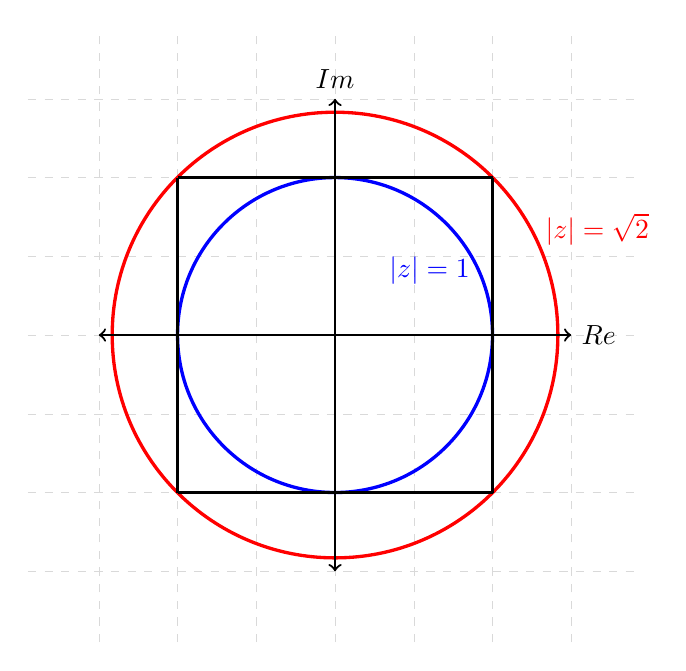
\begin{tikzpicture}
\draw[help lines, color=gray!30, dashed] (-3.9,-3.9) grid (3.9,3.9);
\draw[very thick,red] (2.83,0) arc (0:360:2.83cm) node[above,yshift=1cm,xshift=0.5cm]{$|z|=\sqrt{2}$};
\draw[very thick,blue] (2,0) arc (0:360:2cm) node[above,yshift=0.5cm,xshift=-0.8cm]{$|z|=1$};
\draw[very thick] (-2,-2) -- (2,-2);
\draw[very thick] (-2,-2) -- (-2,2);
\draw[very thick] (2,2) -- (2,-2);
\draw[very thick] (2,2) -- (-2,2);
\draw[<->, thick] (-3,0)--(3,0) node[right]{$Re$};
\draw[<->, thick] (0,-3)--(0,3) node[above]{$Im$};
\end{tikzpicture}
\end{center}

Then on $\{|z|=\sqrt{2}\}$ \begin{align*}
    |f(z)|&\ge |10-i||z|^4-|z|^6-1\\
    &=\sqrt{101}(\sqrt{2})^4-(\sqrt{2})^6-1\\
    &=4\sqrt{101}-8-1\\
    &\ge 40-9\\
    &=31\\
    &>8\\
    &=|-z|^6\\
    &=|g(z)|
\end{align*} and so $|f(z)|>|g(z)|$ so $f(z)$ and $f(z)+g(z)$ have the same number of zeros inside $\{|z|\le\sqrt{2}\}.$

Since $f(z)+g(z)=(10-i)z^4+1$, we need only count the number of zeros of this function. Since if $$(10-i)z^4+1=0\implies z^4=\frac{1}{i-10}\implies |z|^4=\frac{1}{|i-10|}=\frac{1}{\sqrt{101}}<4$$ and so $|z|<\sqrt{2}$. Namely, the zeros of $f+g$ all lie in $\{|z|\le\sqrt{2}\}$ and so $f+g$ and $f$ have four zeros in $\{|z|\le\sqrt{2}\}$.

Now, on $\{|z|=1\}$  \begin{align*}
    |f(z)|&\ge |10-i||z|^4-|z|^6-1\\
    &=\sqrt{101}-1-1\\
    &=\sqrt{101}-2\\
    &> 10-2\\
    &=8\\
    &>8\\
    &=|-z|^6\\
    &=|g(z)|
\end{align*}

And so again, $f(z)$ and $f(z)+g(z)$ have the same number of zeros on $|z|=1.$

Namely, since we already saw $f$ has $4$ zeros in $\{|z|\le\sqrt{2}\}$ and $4$ zeros in $\{|z|\le 1\}$, we have that $f$ has $4$ zeros in the unit square.

Now, we need only show that the zeros of $f$ are all unique.

If $f$ has any repeated roots in the unit square, then $f$ and $f'$ would have a root in common.

Since $f'(z)=6z^5+4(10-i)z^3$ we get that $f'(z)=0$ implies that $2z^3(3z^2+2(10-i))=0$ and since $0$ is not a root of $f$,

the only possibilities are when $z^2=\frac{2i-20}{3}$. However, clearly neither of these roots lie in the unit square, since the largest magnitude inside the unit square is $\sqrt{2}$ (so $|z|^2\le 2$) and $$|\frac{2i-20}{3}|=\frac{\sqrt{2}}{\sqrt{3}}\sqrt{101}>\frac{1}{2}10=5>2.$$

Thus, $f$ and $f'$ share no zeros in the unit square and so $f$ has $4$ distinct zeros inside the unit square.
\end{solution}
\newpage




\begin{problem} $\,$
Suppose that $f$ is holomorphic in a neighborhood $U$ of $a\in\mathbb{C}$. Consider the following two statements:
\begin{enumerate}[label=(\roman*)]
    \item There exist two sequences $\{z_k\}_{k=1}^\infty$ and $\{w_k\}_{k=1}^\infty$ in $U\backslash\{a\}$ converging to $a$ such that $z_k\not=w_k$ and $f(z_k)=f(w_k)$ for all $k\in\mathbb{N}$.
    \item $f'(a)=0$.
\end{enumerate}
Determine whether either of the statements implies the other one. In each case jusifty your answer with a proof or counterexample.
\end{problem}


\begin{solution}$\,$
\boxed{(i)\implies (ii)} True. Assume $f'(z)\not=0.$ Then because $f$ is analytic, the inverse function theorem states that $f$ is invertible in a small neighborhood of $a$. Namely, $f$ must be injective on a small neighborhood of $a$ and so the sequences $\{z_k\}$ and $\{w_k\}$ cannot exist.

Thus, $f'(a)=0$.

\boxed{(i)\impliedby (ii)} Since $f'(a)=0$ WLOG we may take $f(a)=0$ (else we look at $g(z)=f(z)-f(a)$).

Then we can write $f(z)=(z-a)^nh(z)$ where $n\ge 2$ $h(z)$ is analytic in $U$ and nonzero in a neighborhood of $a.$

Since $h$ is analytic, after picking a branch, we can write $f(z)=(g(z))^n$ where $g(z)=(z-a)h^{1/n}(z)$ and $h^{1/n}$ is also analytic and nonzero in a neighborhood of $a.$

Now, by the open mapping theorem, $f(U)$ is open in $\mathbb{C}$ and $0\in f(U).$ Thus, there exists a neighborhood $V$ of $0$ such that $V\subset f(U).$

Namely, $(g(U))^{1/n}$ contains a neighborhood of $0$ and so $re^{2k\pi i/n}\in (g(U))^{1/n}$ for some $r>0$ and $1\le k\le n$.

Namely, $g$ cannot be injective since it wraps some neighborhood of $a$ around the origin $n$-times. Thus, $f$ is also not injective in a neighborhood of $a$ and so (i) is true.
\end{solution}
\newpage





\begin{problem} $\,$
Let $f$ be analytic in an open set $U\subset\mathbb{C}$, and let $K\subset U$ be compact. Show that there exists a constant $C$ depending on $U$ and $K$ such that $$|f(z)|\le C\left(\int_U|f|^2\right)^{1/2}$$
\end{problem}


\begin{solution}$\,$
Let $\{B_r(z)\}_{z\in K}$ be an open cover of $K$. Then by the Lebesgue number lemma, there exists $\delta>0$ such that $B_\delta(z)\subset B_r(z')$ for some $z'\in K$.

\begin{align*}
    |f(z)|&=\left|\frac{1}{2\pi i}\int_{|\xi-z|=\delta}\frac{f(\xi)}{\xi-z}d\xi\right|\\
    &\le \frac{1}{2\pi}\int_{|\xi-z|=\delta}\frac{|f(\xi)|}{|\xi-z|}d|\xi|\\
    &\le \frac{1}{2\pi}\left(\int_{|\xi-z|=\delta}|f(\xi)|^2d|\xi|\right)^{1/2}\left(\int_{|\xi-z|=\delta}\frac{1}{|\xi-z|^2}d|\xi|\right)^{1/2}\qquad\text{Holder's Inequality}\\
    &=\frac{1}{2\pi}\left(\int_{|\xi-z|=\delta}|f(\xi)|^2d|\xi|\right)^{1/2}\left(\int_0^{2\pi}\frac{1}{\delta}d\theta\right)^{1/2}\\
    &=\frac{1}{2\pi}\left(\int_{|\xi-z|=\delta}|f(\xi)|^2d|\xi|\right)^{1/2}\frac{\sqrt{2\pi}}{\sqrt{\delta}}\\
    &=\frac{1}{\sqrt{2\pi\delta}}\left(\int_{|\xi-z|=\delta}|f(\xi)|^2d|\xi|\right)^{1/2}
\end{align*}

\end{solution}


\end{document}
